\section{Sequential Chips}

  Now that we know how the NAND gate---and therefore every other fundamental gate---works, and we have constructed the clock, the next natural step is to be able to store a string of bits.\footnote{Most courses teach combinational logic first and then sequential, but this may not be the most optimal dependency sequence for two reasons. We can indeed do arithmetic without memory by directly applying an electric current to the input wires in a circuit, but this severely limits the computation that we can do. We would essentially have to do everything in ``one shot'' and immediately collect the results. While this is fine for addition, I cannot introduce an efficient schema of multiplication without knowing how to bit-shift, which is dependent on some form of memory. On a broader scale, almost all algorithms we worked with require some memory at some point, so memory may be more fundamental than computation.} Computers must be equipped with memory elements that can preserve data over time. These memory elements are built from \textit{sequential chips}. 

\subsection{Latches}

  Ideally, we would like a way to store a bit in memory, and this can be done by cross-coupling gates with each other, forming a sort of positive feedback.\footnote{Note that unlike combinational logic, this now deviates from straight-line programming.} Therefore, given a certain signal into our circuit which we call a \textit{latch}, the outputs remain locked---or ``latched''---into a state. 

  \begin{definition}[SR Latch]
    The \textbf{set-reset (SR) latch} is a circuit that stores 1-bit memory. This is based on \textit{pulses} and we do not care about the duration of a signal. That is, if we activate a signal to inputs $S, R$ at \textit{any} point in time, then the output $Q$ will remain locked in some state, even \textit{after} the input signal disappears. 
  \end{definition}

  The SR latch---like all electronic circuits---require power to work, labeled with $S$ and $R$. The output is really just $Q$, but we can add redundancy by making the inverse $\overline{Q}$ available as well. There are two implementations of an SR latch, which have symmetric behaviors. 

  \begin{theorem}[Active High SR Latch]
    A NOR SR latch can be implemented in the following circuit below, with its corresponding truth table. 

    \begin{figure}[H]
      \centering
      \begin{subfigure}[b]{0.48\textwidth}
        \centering
        \begin{tikzpicture}[circuit logic US]
          \node[nor gate] (nor1) at (0, 1) {}; 
          \node[nor gate] (nor2) at (0, -1) {}; 

          \node[left] at (-1.5, 1.1) {$S$}; 
          \node[left] at (-1.5, -1.1) {$R$}; 
          \node[right] at (2, 1) {$Q$};
          \node[right] at (2, -1) {$\overline{Q}$};

          \draw (-1.5, 1.1) -| (nor1.input 1);
          \draw (-1.5, -1.1) -| (nor2.input 2);
          \draw (nor1.output) |- (2, 1); 
          \draw (nor2.output) |- (2, -1); 

          \draw (nor1.output) |- (1.5, 1) -- (1.5, 0.8) -- (-1, -0.7) -- (-1, -0.9) |- (nor2.input 1);
          \draw (nor2.output) |- (1.5, -1) -- (1.5, -0.8) -- (-1, 0.7) -- (-1, 0.9) |- (nor1.input 2);
          \fill (1.5,1) circle (1.5pt);
          \fill (1.5,-1) circle (1.5pt);
        \end{tikzpicture} 
        \caption{Circuit diagram.}
      \end{subfigure}
      \hfill 
      \begin{subfigure}[b]{0.48\textwidth}
        \centering
        \begin{tabular}{|c|c|c|c|}
          \hline
          \textbf{S} & \textbf{R} & \textbf{Q} & \textbf{$\overline{Q}$} \\
          \hline
          0 & 0 & 1 & 0 \\
            &   & 0 & 1 \\
          \hline
          0 & 1 & 0 & 1 \\
          \hline
          1 & 0 & 1 & 0 \\
          \hline
          1 & 1 & 0 & 0 \\
          \hline
        \end{tabular} 
        \caption{Truth table.}
      \end{subfigure}
      \caption{XOR SR Latch. This is }
    \end{figure}

    Setting both $R = S = 1$ would result in an invalid state since they would attempt to turn $Q$ back and forth between $0$ and $1$, giving us a race condition. 

    \begin{figure}[H]
      \centering
      \begin{subfigure}[b]{0.48\textwidth}
        \centering
        \begin{tikzpicture}[circuit logic US]
          \node[nor gate] (nor1) at (0, 1) {}; 
          \node[nor gate] (nor2) at (0, -1) {}; 

          \node[left] at (-1.5, 1.1) {$S$}; 
          \node[left] at (-1.5, -1.1) {$R$}; 
          \node[right] at (2, 1) {$Q$};
          \node[right] at (2, -1) {$\overline{Q}$};

          \draw[blue] (-1.5, 1.1) -| (nor1.input 1);
          \draw[blue] (-1.5, -1.1) -| (nor2.input 2);
          \draw[red] (nor1.output) |- (2, 1); 
          \draw[blue] (nor2.output) |- (2, -1); 

          \draw[red] (nor1.output) |- (1.5, 1) -- (1.5, 0.8) -- (-1, -0.7) -- (-1, -0.9) |- (nor2.input 1);
          \draw[blue] (nor2.output) |- (1.5, -1) -- (1.5, -0.8) -- (-1, 0.7) -- (-1, 0.9) |- (nor1.input 2);
          \fill[red] (1.5,1) circle (1.5pt);
          \fill[blue] (1.5,-1) circle (1.5pt);
        \end{tikzpicture} 
        \caption{}
      \end{subfigure}
      \hfill 
      \begin{subfigure}[b]{0.48\textwidth}
        \centering
        \begin{tikzpicture}[circuit logic US]
          \node[nor gate] (nor1) at (0, 1) {}; 
          \node[nor gate] (nor2) at (0, -1) {}; 

          \node[left] at (-1.5, 1.1) {$S$}; 
          \node[left] at (-1.5, -1.1) {$R$}; 
          \node[right] at (2, 1) {$Q$};
          \node[right] at (2, -1) {$\overline{Q}$};

          \draw[blue] (-1.5, 1.1) -| (nor1.input 1);
          \draw[blue] (-1.5, -1.1) -| (nor2.input 2);
          \draw[blue] (nor1.output) |- (2, 1); 
          \draw[red] (nor2.output) |- (2, -1); 

          \draw[blue] (nor1.output) |- (1.5, 1) -- (1.5, 0.8) -- (-1, -0.7) -- (-1, -0.9) |- (nor2.input 1);
          \draw[red] (nor2.output) |- (1.5, -1) -- (1.5, -0.8) -- (-1, 0.7) -- (-1, 0.9) |- (nor1.input 2);
          \fill[blue] (1.5,1) circle (1.5pt);
          \fill[red] (1.5,-1) circle (1.5pt);
        \end{tikzpicture} 
        \caption{}
      \end{subfigure}
      \caption{Two possible initial states. The default state is $R = 0, S = 0$, which are both \textit{low states}, and $Q$ may be either $0$ or $1$. }
    \end{figure}

    If one of $R$ or $S$ is set to a high state, the latch is activated, and hence this is called an \textbf{active high SR latch}. Note that regardless of what the previous state the latch was in, the output signals are completely determined. 

    \begin{figure}[H]
      \centering
      \begin{subfigure}[b]{0.48\textwidth}
        \centering
        \begin{tikzpicture}[circuit logic US]
          \node[nor gate] (nor1) at (0, 1) {}; 
          \node[nor gate] (nor2) at (0, -1) {}; 

          \node[left] at (-1.5, 1.1) {$S$}; 
          \node[left] at (-1.5, -1.1) {$R$}; 
          \node[right] at (2, 1) {$Q$};
          \node[right] at (2, -1) {$\overline{Q}$};

          \draw[red] (-1.5, 1.1) -| (nor1.input 1);
          \draw[blue] (-1.5, -1.1) -| (nor2.input 2);
          \draw[blue] (nor1.output) |- (2, 1); 
          \draw[red] (nor2.output) |- (2, -1); 

          \draw[blue] (nor1.output) |- (1.5, 1) -- (1.5, 0.8) -- (-1, -0.7) -- (-1, -0.9) |- (nor2.input 1);
          \draw[red] (nor2.output) |- (1.5, -1) -- (1.5, -0.8) -- (-1, 0.7) -- (-1, 0.9) |- (nor1.input 2);
          \fill[blue] (1.5,1) circle (1.5pt);
          \fill[red] (1.5,-1) circle (1.5pt);
        \end{tikzpicture} 
        \caption{If we send a signal $R = 1$, then $Q = 0$, and even if we reset $R = 0$, $Q$ is still locked at $0$. }
      \end{subfigure}
      \hfill 
      \begin{subfigure}[b]{0.48\textwidth}
        \centering
        \begin{tikzpicture}[circuit logic US]
          \node[nor gate] (nor1) at (0, 1) {}; 
          \node[nor gate] (nor2) at (0, -1) {}; 

          \node[left] at (-1.5, 1.1) {$S$}; 
          \node[left] at (-1.5, -1.1) {$R$}; 
          \node[right] at (2, 1) {$Q$};
          \node[right] at (2, -1) {$\overline{Q}$};

          \draw[blue] (-1.5, 1.1) -| (nor1.input 1);
          \draw[red] (-1.5, -1.1) -| (nor2.input 2);
          \draw[red] (nor1.output) |- (2, 1); 
          \draw[blue] (nor2.output) |- (2, -1); 

          \draw[red] (nor1.output) |- (1.5, 1) -- (1.5, 0.8) -- (-1, -0.7) -- (-1, -0.9) |- (nor2.input 1);
          \draw[blue] (nor2.output) |- (1.5, -1) -- (1.5, -0.8) -- (-1, 0.7) -- (-1, 0.9) |- (nor1.input 2);
          \fill[red] (1.5,1) circle (1.5pt);
          \fill[blue] (1.5,-1) circle (1.5pt);
        \end{tikzpicture} 
        \caption{If we send a signal $S = 1$, then $Q = 1$, and even if reset $S = 0$, $Q$ is still locked at $1$. }
      \end{subfigure}
      \caption{}
    \end{figure}
  \end{theorem}

  Now unlike the active high latches which are activated when the current is $1$, active low latches are activated when the current is $0$. 

  \begin{theorem}[Active Low SR Latch]
    A NAND SR latch can be implemented in the following circuit below, with its corresponding truth table. 
    
    \begin{figure}[H]
      \centering
      \begin{subfigure}[b]{0.48\textwidth}
        \centering
        \begin{tikzpicture}[circuit logic US]
          \node[nand gate] (nor1) at (0, 1) {}; 
          \node[nand gate] (nor2) at (0, -1) {}; 
          \node[left] at (-1.5, 1.1) {$S$}; 
          \node[left] at (-1.5, -1.1) {$R$}; 
          \node[right] at (2, 1) {$Q$};
          \node[right] at (2, -1) {$\overline{Q}$};

          \draw (-1.5, 1.1) -| (nor1.input 1);
          \draw (-1.5, -1.1) -| (nor2.input 2);
          \draw (nor1.output) |- (2, 1); 
          \draw (nor2.output) |- (2, -1); 

          \draw (nor1.output) |- (1.5, 1) -- (1.5, 0.8) -- (-1, -0.7) -- (-1, -0.9) |- (nor2.input 1);
          \draw (nor2.output) |- (1.5, -1) -- (1.5, -0.8) -- (-1, 0.7) -- (-1, 0.9) |- (nor1.input 2);
          \fill (1.5,1) circle (1.5pt);
          \fill (1.5,-1) circle (1.5pt);
        \end{tikzpicture} 
        \caption{Circuit diagram.}
      \end{subfigure}
      \hfill 
      \begin{subfigure}[b]{0.48\textwidth}
        \centering
        \begin{tabular}{|c|c|c|c|}
          \hline
          \textbf{S} & \textbf{R} & \textbf{Q} & \textbf{$\overline{Q}$} \\
          \hline
          0 & 0 & 1 & 1 \\
          \hline
          0 & 1 & 1 & 0 \\
          \hline
          1 & 0 & 0 & 1 \\
          \hline
          1 & 1 & 0 & 1 \\
            &   & 1 & 0 \\
          \hline
        \end{tabular}
        \caption{Truth table.}
      \end{subfigure}
      \caption{NAND SR Latch}
    \end{figure}

    Setting both $R = S = 0$ would result in an invalid state since they would attempt to turn $Q$ back and forth between $0$ and $1$, giving us a race condition. 

    \begin{figure}[H]
      \centering
      \begin{subfigure}[b]{0.48\textwidth}
        \centering
        \begin{tikzpicture}[circuit logic US]
          \node[nand gate] (nor1) at (0, 1) {}; 
          \node[nand gate] (nor2) at (0, -1) {}; 
          \node[left] at (-1.5, 1.1) {$S$}; 
          \node[left] at (-1.5, -1.1) {$R$}; 
          \node[right] at (2, 1) {$Q$};
          \node[right] at (2, -1) {$\overline{Q}$};

          \draw[red] (-1.5, 1.1) -- (nor1.input 1);
          \draw[red] (-1.5, -1.1) -- (nor2.input 2);
          \draw[blue] (nor1.output) -- (2, 1); 
          \draw[red] (nor2.output) -- (2, -1); 

          \draw[blue] (nor1.output) -- (1.5, 1) -- (1.5, 0.8) -- (-1, -0.7) -- (-1, -0.9) -- (nor2.input 1);
          \draw[red] (nor2.output) -- (1.5, -1) -- (1.5, -0.8) -- (-1, 0.7) -- (-1, 0.9) -- (nor1.input 2);
          \fill[blue] (1.5,1) circle (1.5pt);
          \fill[red] (1.5,-1) circle (1.5pt);
        \end{tikzpicture} 
        \caption{}
      \end{subfigure}
      \hfill 
      \begin{subfigure}[b]{0.48\textwidth}
        \centering
        \begin{tikzpicture}[circuit logic US]
          \node[nand gate] (nor1) at (0, 1) {}; 
          \node[nand gate] (nor2) at (0, -1) {}; 
          \node[left] at (-1.5, 1.1) {$S$}; 
          \node[left] at (-1.5, -1.1) {$R$}; 
          \node[right] at (2, 1) {$Q$};
          \node[right] at (2, -1) {$\overline{Q}$};

          \draw[red] (-1.5, 1.1) -- (nor1.input 1);
          \draw[red] (-1.5, -1.1) -- (nor2.input 2);
          \draw[red] (nor1.output) -- (2, 1); 
          \draw[blue] (nor2.output) -- (2, -1); 

          \draw[red] (nor1.output) -- (1.5, 1) -- (1.5, 0.8) -- (-1, -0.7) -- (-1, -0.9) -- (nor2.input 1);
          \draw[blue] (nor2.output) -- (1.5, -1) -- (1.5, -0.8) -- (-1, 0.7) -- (-1, 0.9) -- (nor1.input 2);
          \fill[red] (1.5,1) circle (1.5pt);
          \fill[blue] (1.5,-1) circle (1.5pt);
        \end{tikzpicture} 
        \caption{}
      \end{subfigure}
      \caption{The default state is $R = 1, S = 1$, i.e. they are both \textit{high states}, and $Q$ may be either $0$ or $1$. This is known as an \textbf{active low SR latch}. }
    \end{figure}

    If one of $R$ or $S$ is set to a low state, the latch is activated, and hence this is called an \textbf{active low SR latch}. Note that regardless of what the previous state the latch was in, the output signals are completely determined. 

    \begin{figure}[H]
      \centering
      \begin{subfigure}[b]{0.48\textwidth}
        \centering
        \begin{tikzpicture}[circuit logic US]
          \node[nand gate] (nor1) at (0, 1) {}; 
          \node[nand gate] (nor2) at (0, -1) {}; 
          \node[left] at (-1.5, 1.1) {$S$}; 
          \node[left] at (-1.5, -1.1) {$R$}; 
          \node[right] at (2, 1) {$Q$};
          \node[right] at (2, -1) {$\overline{Q}$};

          \draw[blue] (-1.5, 1.1) -| (nor1.input 1);
          \draw[red] (-1.5, -1.1) -| (nor2.input 2);
          \draw[red] (nor1.output) |- (2, 1); 
          \draw[blue] (nor2.output) |- (2, -1); 

          \draw[red] (nor1.output) |- (1.5, 1) -- (1.5, 0.8) -- (-1, -0.7) -- (-1, -0.9) |- (nor2.input 1);
          \draw[blue] (nor2.output) |- (1.5, -1) -- (1.5, -0.8) -- (-1, 0.7) -- (-1, 0.9) |- (nor1.input 2);
          \fill[red] (1.5,1) circle (1.5pt);
          \fill[blue] (1.5,-1) circle (1.5pt);
        \end{tikzpicture} 
        \caption{}
      \end{subfigure}
      \hfill 
      \begin{subfigure}[b]{0.48\textwidth}
        \centering
        \begin{tikzpicture}[circuit logic US]
          \node[nand gate] (nor1) at (0, 1) {}; 
          \node[nand gate] (nor2) at (0, -1) {}; 
          \node[left] at (-1.5, 1.1) {$S$}; 
          \node[left] at (-1.5, -1.1) {$R$}; 
          \node[right] at (2, 1) {$Q$};
          \node[right] at (2, -1) {$\overline{Q}$};

          \draw[red] (-1.5, 1.1) -| (nor1.input 1);
          \draw[blue] (-1.5, -1.1) -| (nor2.input 2);
          \draw[blue] (nor1.output) |- (2, 1); 
          \draw[red] (nor2.output) |- (2, -1); 

          \draw[blue] (nor1.output) |- (1.5, 1) -- (1.5, 0.8) -- (-1, -0.7) -- (-1, -0.9) |- (nor2.input 1);
          \draw[red] (nor2.output) |- (1.5, -1) -- (1.5, -0.8) -- (-1, 0.7) -- (-1, 0.9) |- (nor1.input 2);
          \fill[blue] (1.5,1) circle (1.5pt);
          \fill[red] (1.5,-1) circle (1.5pt);
        \end{tikzpicture} 
        \caption{}
      \end{subfigure}
      \caption{If we send a signal $S = 0$, then $Q = 0$, and even if reset $S = 1$, $Q$ is still locked at $0$. }
    \end{figure}
  \end{theorem}

  These signals may be noisy, and we might want more control over whether a latch can change states, i.e its \textit{transparency}. This is done by adding an extra \textit{gate} that explicitly tells us when the latch can change states. 

  \begin{definition}[Gated SR Latch]
    A \textbf{gated SR latch} is an SR latch that can only change state when it is enabled. This enabling is done with an additional 2 NAND gates, and so the SR latch is enabled only when $E = 1$. 

    \begin{figure}[H]
      \centering
      \begin{subfigure}[b]{0.48\textwidth}
        \centering
        \begin{tikzpicture}[circuit logic US]
          \node[nand gate] (nand1) at (-2, 1.1) {};
          \node[nand gate] (nand2) at (-2, -1.1) {};
          \node[nor gate] (nor1) at (0, 1) {}; 
          \node[nor gate] (nor2) at (0, -1) {}; 

          \draw (-3, 1.2) -- (nand1.input 1);
          \draw (-3, -1.2) -- (nand2.input 2);
          \draw (-3, 0) -- (-2.7, 0) -- (-2.7,1) -- (nand1.input 2);
          \draw (-3, 0) -- (-2.7, 0) -- (-2.7,-1) -- (nand2.input 1);
          \node[left] at (-3,0) {$E$};
          \node[left] at (-3,1.2) {$S$};
          \node[left] at (-3,-1.2) {$R$};
          \node[right] at (2, 1) {$Q$};
          \node[right] at (2, -1) {$\overline{Q}$};

          \draw (nand1.output) -- (nor1.input 1);
          \draw (nand2.output) -- (nor2.input 2);
          \draw (nor1.output) -- (2, 1); 
          \draw (nor2.output) -- (2, -1); 

          \draw (nor1.output) -- (1.5, 1) -- (1.5, 0.8) -- (-1, -0.7) -- (-1, -0.9) -- (nor2.input 1);
          \draw (nor2.output) -- (1.5, -1) -- (1.5, -0.8) -- (-1, 0.7) -- (-1, 0.9) -- (nor1.input 2);
          \fill (1.5,1) circle (1.5pt);
          \fill (1.5,-1) circle (1.5pt);
          \fill (-2.7,0) circle (1.5pt);
        \end{tikzpicture} 
        \caption{Gated XOR SR Latch.}
      \end{subfigure}
      \hfill 
      \begin{subfigure}[b]{0.48\textwidth}
        \centering
        \begin{tikzpicture}[circuit logic US]
          \node[nand gate] (nand1) at (-2, 1.1) {};
          \node[nand gate] (nand2) at (-2, -1.1) {};
          \node[nand gate] (nor1) at (0, 1) {}; 
          \node[nand gate] (nor2) at (0, -1) {}; 

          \draw (-3, 1.2) -- (nand1.input 1);
          \draw (-3, -1.2) -- (nand2.input 2);
          \draw (-3, 0) -- (-2.7, 0) -- (-2.7,1) -- (nand1.input 2);
          \draw (-3, 0) -- (-2.7, 0) -- (-2.7,-1) -- (nand2.input 1);
          \node[left] at (-3,0) {$E$};
          \node[left] at (-3,1.2) {$S$};
          \node[left] at (-3,-1.2) {$R$};
          \node[right] at (2, 1) {$Q$};
          \node[right] at (2, -1) {$\overline{Q}$};

          \draw (nand1.output) -- (nor1.input 1);
          \draw (nand2.output) -- (nor2.input 2);
          \draw (nor1.output) -- (2, 1); 
          \draw (nor2.output) -- (2, -1); 

          \draw (nor1.output) -- (1.5, 1) -- (1.5, 0.8) -- (-1, -0.7) -- (-1, -0.9) -- (nor2.input 1);
          \draw (nor2.output) -- (1.5, -1) -- (1.5, -0.8) -- (-1, 0.7) -- (-1, 0.9) -- (nor1.input 2);
          \fill (1.5,1) circle (1.5pt);
          \fill (1.5,-1) circle (1.5pt);
          \fill (-2.7,0) circle (1.5pt);
        \end{tikzpicture} 
        \caption{Gated NAND SR Latch.}
      \end{subfigure}
      \caption{Note that if $E = 0$, then the output of the leftmost two NAND gates will be $1$ no matter what, and so the values of $R, S$ does not have any effect. }
    \end{figure}
  \end{definition}

  \begin{example}[Active High Gated SR Latch]
    By keeping track of the voltages in the wires of interest and running them across a common time axis, we can visualize this circuit in action. Note that in here, we assume that electric current is instantaneous, resulting in the familiar \textit{square waves}. Let's look at an active high SR latch. 

    \begin{figure}[H]
      \centering 
      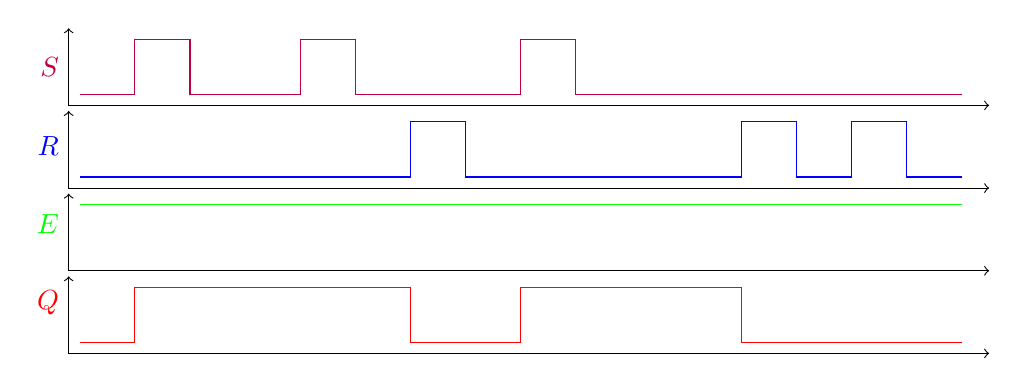
\begin{tikzpicture}[scale=0.7]
        \def\h{1.5}
        \draw[<->] (-0.2, 1.2) -- (-0.2, -0.2) -- (16.5, -0.2); 
        \draw[<->, yshift=-1.5cm] (-0.2, 1.2) -- (-0.2, -0.2) -- (16.5, -0.2); 
        \draw[<->, yshift=-3cm] (-0.2, 1.2) -- (-0.2, -0.2) -- (16.5, -0.2); 
        \draw[<->, yshift=-4.5cm] (-0.2, 1.2) -- (-0.2, -0.2) -- (16.5, -0.2); 
        \node[purple, left] at (-0.2, 0.5) {$S$}; 
        \node[blue, left, yshift=-1cm] at (-0.2, 0.5) {$R$}; 
        \node[green, left, yshift=-2cm] at (-0.2, 0.5) {$E$}; 
        \node[red, left, yshift=-3cm] at (-0.2, 0.5) {$Q$}; 

        \draw[purple] (0, 0) -- (1, 0) -- (1, 1) -- (2, 1) -- (2, 0) -- (4, 0) -- (4, 1) -- (5, 1) -- (5, 0) -- (8, 0) -- (8, 1) -- (9, 1) -- (9, 0) -- (16, 0);
        \draw[blue, yshift=-1.5cm] (0, 0) -- (6, 0) -- (6, 1) -- (7, 1) -- (7, 0) -- (12, 0) -- (12, 1) -- (13, 1) -- (13, 0) -- (14, 0) -- (14, 1) -- (15, 1) -- (15, 0) -- (16, 0);
        \draw[green, yshift=-3cm] (0, 1) -- (16, 1);
        \draw[red, yshift=-4.5cm] (0, 0) -- (1, 0) -- (1, 1) -- (6, 1) -- (6, 0) -- (8, 0) -- (8, 1) -- (12, 1) -- (12, 0) -- (16, 0);
      \end{tikzpicture}
      \caption{In here the gate is always enabled as $E = 1$ always. In the beginning $S = 1$ causing $Q = 1$, and this does not change until $R = 1$, at which point $Q = 0$. Note that the second pulse of $S$ does not affect the state because it is already $Q = 1$. Soon after $S = 1$ again, causing $Q = 1$ and when $R = 1$ $Q = 0$.}
    \end{figure}

    \begin{figure}[H]
      \centering 
      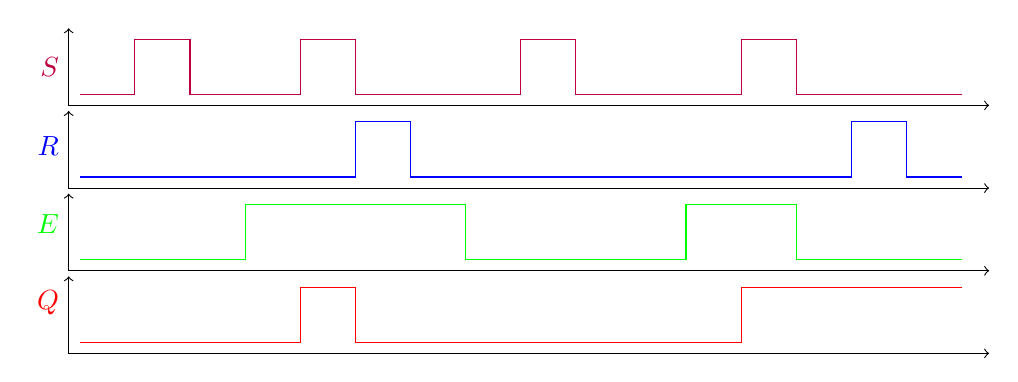
\begin{tikzpicture}[scale=0.7]
        \draw[<->] (-0.2, 1.2) -- (-0.2, -0.2) -- (16.5, -0.2); 
        \draw[<->, yshift=-1.5cm] (-0.2, 1.2) -- (-0.2, -0.2) -- (16.5, -0.2); 
        \draw[<->, yshift=-3cm] (-0.2, 1.2) -- (-0.2, -0.2) -- (16.5, -0.2); 
        \draw[<->, yshift=-4.5cm] (-0.2, 1.2) -- (-0.2, -0.2) -- (16.5, -0.2); 
        \node[purple, left] at (-0.2, 0.5) {$S$}; 
        \node[blue, left, yshift=-1cm] at (-0.2, 0.5) {$R$}; 
        \node[green, left, yshift=-2cm] at (-0.2, 0.5) {$E$}; 
        \node[red, left, yshift=-3cm] at (-0.2, 0.5) {$Q$}; 

        \draw[purple] (0, 0) -- 
          (1, 0) -- (1, 1) -- (2, 1) -- (2, 0) -- 
          (4, 0) -- (4, 1) -- (5, 1) -- (5, 0) -- 
          (8, 0) -- (8, 1) -- (9, 1) -- (9, 0) -- 
          (12, 0) -- (12, 1) -- (13, 1) -- (13, 0) -- 
          (16, 0);
        \draw[blue, yshift=-1.5cm] (0, 0) -- 
          (5, 0) -- (5, 1) -- (6, 1) -- (6, 0) -- 
          (14, 0) -- (14, 1) -- (15, 1) -- (15, 0) -- 
          (16, 0);
        \draw[green, yshift=-3cm] (0, 0) -- 
          (3, 0) -- (3, 1) -- (7, 1) -- (7, 0) -- 
          (11, 0) -- (11, 1) -- (13, 1) -- (13, 0) -- 
          (16, 0);
        \draw[red, yshift=-4.5cm] (0, 0) -- 
          (4, 0) -- (4, 1) -- (5, 1) -- (5, 0) -- 
          (12, 0) -- (12, 1) -- (16, 1);
      \end{tikzpicture}
      \caption{Now we toggle $E$ on and off throughout. We can start off by filling in all the places where $E = 1$, where we want $Q$ to basically copy $S$. At every other place, we just continue what the state $Q$ was in. } 
    \end{figure}
  \end{example}

  Note that we still have the problem of invalid signals. For example, if there was an instance that at the same clock time a signal of $S=1, R=1$ (on either an ungated latch or a gated latch with $E=1$), then both $Q$ and $\overline{Q}$ will be $1$, which will cause both to be $0$, and then $1$, and so on. This causes a race condition, which leads to unpredictable behavior. 

  \begin{figure}[H]
    \centering 
    \begin{tikzpicture}[circuit logic US]
      \node[nand gate] (nand1) at (-2, 1.1) {};
      \node[nand gate] (nand2) at (-2, -1.1) {};
      \node[nor gate] (nor1) at (0, 1) {}; 
      \node[nor gate] (nor2) at (0, -1) {}; 
      \node[not gate, point down, scale=0.8] (not1) at (-3.5, 0.8) {};

      \draw (-4, 1.2) -- (nand1.input 1);
      \draw (-4, 1.2) -- (-3.5, 1.2) -- (not1.input); 
      \draw (not1.output) -- (-3.5, 0.1) -- (-3.4, 0) -- (-3.5, -0.1) -- (-3.5, -1.2) -- (nand2.input 2);
      \draw (-4, 0) -- (-2.7, 0) -- (-2.7,1) -- (nand1.input 2);
      \draw (-4, 0) -- (-2.7, 0) -- (-2.7,-1) -- (nand2.input 1);
      \node[left] at (-4,0) {$E$};
      \node[left] at (-4,1.2) {$D$};
      \node[right] at (2, 1) {$Q$};
      \node[right] at (2, -1) {$\overline{Q}$};

      \draw (nand1.output) -- (nor1.input 1);
      \draw (nand2.output) -- (nor2.input 2);
      \draw (nor1.output) -- (2, 1); 
      \draw (nor2.output) -- (2, -1); 

      \draw (nor1.output) -- (1.5, 1) -- (1.5, 0.8) -- (-1, -0.7) -- (-1, -0.9) -- (nor2.input 1);
      \draw (nor2.output) -- (1.5, -1) -- (1.5, -0.8) -- (-1, 0.7) -- (-1, 0.9) -- (nor1.input 2);
      \fill (1.5,1) circle (1.5pt);
      \fill (1.5,-1) circle (1.5pt);
      \fill (-2.7,0) circle (1.5pt);
    \end{tikzpicture} 
    \caption{} 
  \end{figure}

  It turns out that we can simplify this circuit, making it cheaper to produce while still behaving identically. This gives us the D-latch. 

  \begin{definition}[D Latch]
    The \textbf{(gated) data latch (D-latch)} gives us more control over storing a 1-bit in memory. 

    \begin{figure}[H]
      \centering
      \begin{subfigure}[b]{0.48\textwidth}
        \centering
        \begin{tikzpicture}
          \node[latch, align=center] (latch) at (0,0) {D Latch};
          \draw (latch.pin 1) -- ++(-0.5,0) node[left] {D};
          \draw (latch.pin 3) -- ++(-0.5,0) node[left] {E};
          \draw (latch.pin 6) -- ++(0.5,0) node[right] {Q};
          \draw (latch.pin 4) -- ++(0.5,0) node[right] {$\overline{Q}$};
        \end{tikzpicture}
        \caption{Chip notation for D latch.}
      \end{subfigure}
      \hfill 
      \begin{subfigure}[b]{0.48\textwidth}
        \centering
          \begin{tabular}{|c|c|c|c|}
            \hline
            $E$ & $D$ & $Q$ & $\overline{Q}$ \\
            \hline
            0 & X & $Q_{\mathrm{prev}}$ & $\overline{Q_{\mathrm{prev}}}$ \\
            \hline
            1 & 0 & 0 & 1 \\
            \hline
            1 & 1 & 1 & 0 \\
            \hline
          \end{tabular}
        \caption{Truth table. Note that the }
      \end{subfigure}
      \caption{}
    \end{figure}

    \begin{figure}[H]
      \centering
      \begin{subfigure}[b]{0.48\textwidth}
        \centering
        \begin{tikzpicture}[circuit logic US]
          \node[nand gate] (nand1) at (-2, 1.1) {};
          \node[nand gate] (nand2) at (-2, -1.1) {};
          \node[nor gate] (nor1) at (0, 1) {}; 
          \node[nor gate] (nor2) at (0, -1) {}; 

          \draw (-3.5, 1.2) -- (nand1.input 1);
          \draw (-3.5, -1.2) -- (nand2.input 2);
          \node[left] at (-3.5,-1.2) {$E$};
          \node[left] at (-3.5,1.2) {$R$};
          \node[right] at (2, 1) {$Q$};
          \node[right] at (2, -1) {$\overline{Q}$};

          \draw (-3.5, -1.2) -- (-3.2, -1.2) -- (-3.2, 1) -- (nand1.input 2);
          \fill (-3.2, -1.2) circle (1.5pt);
          \draw (nand1.output) -- (-1.2, 1.1) -- (-1.2, 0.9) -- (-2.7, -0.9) -- (-2.7, -1) -- (nand2.input 1);

          \draw (nand1.output) -- (nor1.input 1);
          \draw (nand2.output) -- (nor2.input 2);
          \draw (nor1.output) -- (2, 1); 
          \draw (nor2.output) -- (2, -1); 

          \draw (nor1.output) -- (1.5, 1) -- (1.5, 0.8) -- (-1, -0.7) -- (-1, -0.9) -- (nor2.input 1);
          \draw (nor2.output) -- (1.5, -1) -- (1.5, -0.8) -- (-1, 0.7) -- (-1, 0.9) -- (nor1.input 2);
          \fill (1.5,1) circle (1.5pt);
          \fill (1.5,-1) circle (1.5pt);
        \end{tikzpicture} 
        \caption{Gated XOR SR Latch.}
      \end{subfigure}
      \hfill 
      \begin{subfigure}[b]{0.48\textwidth}
        \centering
        \begin{tikzpicture}[circuit logic US]
          \node[nand gate] (nand1) at (-2, 1.1) {};
          \node[nand gate] (nand2) at (-2, -1.1) {};
          \node[nand gate] (nor1) at (0, 1) {}; 
          \node[nand gate] (nor2) at (0, -1) {}; 

          \draw (-3.5, 1.2) -- (nand1.input 1);
          \draw (-3.5, -1.2) -- (nand2.input 2);
          \node[left] at (-3.5,-1.2) {$E$};
          \node[left] at (-3.5,1.2) {$R$};
          \node[right] at (2, 1) {$Q$};
          \node[right] at (2, -1) {$\overline{Q}$};

          \draw (-3.5, -1.2) -- (-3.2, -1.2) -- (-3.2, 1) -- (nand1.input 2);
          \fill (-3.2, -1.2) circle (1.5pt);
          \draw (nand1.output) -- (-1.2, 1.1) -- (-1.2, 0.9) -- (-2.7, -0.9) -- (-2.7, -1) -- (nand2.input 1);

          \draw (nand1.output) -- (nor1.input 1);
          \draw (nand2.output) -- (nor2.input 2);
          \draw (nor1.output) -- (2, 1); 
          \draw (nor2.output) -- (2, -1); 

          \draw (nor1.output) -- (1.5, 1) -- (1.5, 0.8) -- (-1, -0.7) -- (-1, -0.9) -- (nor2.input 1);
          \draw (nor2.output) -- (1.5, -1) -- (1.5, -0.8) -- (-1, 0.7) -- (-1, 0.9) -- (nor1.input 2);
          \fill (1.5,1) circle (1.5pt);
          \fill (1.5,-1) circle (1.5pt);
        \end{tikzpicture} 
        \caption{Gated NAND SR Latch.}
      \end{subfigure}
      \caption{}
    \end{figure}
  \end{definition}

  \begin{example}[D Latch]
    The essence of the behavior is the output follows the input while $E$ is enabled. 

    \begin{figure}[H]
      \centering 
      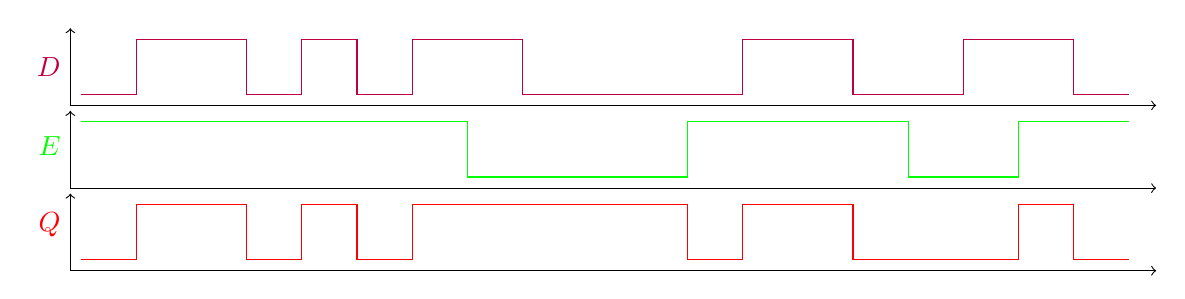
\begin{tikzpicture}[scale=0.7]
        \draw[<->] (-0.2, 1.2) -- (-0.2, -0.2) -- (19.5, -0.2); 
        \draw[<->, yshift=-1.5cm] (-0.2, 1.2) -- (-0.2, -0.2) -- (19.5, -0.2); 
        \draw[<->, yshift=-3cm] (-0.2, 1.2) -- (-0.2, -0.2) -- (19.5, -0.2); 
        \node[purple, left] at (-0.2, 0.5) {$D$}; 
        \node[green, left, yshift=-1cm] at (-0.2, 0.5) {$E$}; 
        \node[red, left, yshift=-2cm] at (-0.2, 0.5) {$Q$}; 

        \draw[purple] (0, 0) -- 
          (1, 0) -- (1, 1) -- (3, 1) -- (3, 0) -- 
          (4, 0) -- (4, 1) -- (5, 1) -- (5, 0) -- 
          (6, 0) -- (6, 1) -- (8, 1) -- (8, 0) -- 
          (12, 0) -- (12, 1) -- (14, 1) -- (14, 0) -- 
          (16, 0) -- (16, 1) -- (18, 1) -- (18, 0) -- 
          (19, 0);
        \draw[green, yshift=-1.5cm] 
          (0, 1) --  (7, 1) -- (7, 0) -- 
          (11, 0) -- (11, 1) -- (15, 1) -- (15, 0) -- 
          (17, 0) -- (17, 1) -- (19, 1);
        \draw[red, yshift=-3cm] (0, 0) -- 
          (1, 0) -- (1, 1) -- (3, 1) -- (3, 0) -- 
          (4, 0) -- (4, 1) -- (5, 1) -- (5, 0) -- 
          (6, 0) -- (6, 1) -- (11, 1) -- (11, 0) -- 
          (12, 0) -- (12, 1) -- (14, 1) -- (14, 0) -- 
          (17, 0) -- (17, 1) -- (18, 1) -- (18, 0) -- 
          (19, 0);
      \end{tikzpicture}
      \caption{Again, we just let the result $Q$ follow the input $D$ whenever $E = 1$,and continue the rest for when $E = 0$.}
    \end{figure}
  \end{example} 

  Therefore, if we want to store a bit of information, we set $E = 1$, collect that bit from $D$, and then set $E = 0$ to latch it in place. 

\subsection{Clocked Latches}

  This behavior is quite stable for storing 1-bit, but we need more control when storing a multi-bit buffer, where we need several D-latches working in tandem. The general idea is that if we have a multi-bit buffer, we want a set of D-latches to be enabled and disabled at once. 

  \begin{figure}[H]
    \centering 
    \begin{tikzpicture}
      \foreach \h in {0, 2, 4} {
        \draw (0, 0+\h) rectangle (0.8, 1.2+\h);
        \draw (-3, 1+\h) -- (0, 1+\h); 
        \draw (0.8, 0.65+\h) -- (2, 0.65+\h); 
        \node[right, font=\footnotesize] at (0, 1+\h) {$D$};
        \node[left, font=\footnotesize] at (0.8, 0.65+\h) {$Q$};
        \node[right, font=\footnotesize] at (0, 0.3+\h) {$E$};
        \draw (-1, 0.3+\h) -- (0, 0.3+\h);
        \fill (-1, 0.3+\h) circle (1.5pt);
      }
      \node[draw, circle] (clock) at (-4, -1) {clock};
      \draw (clock.east) -- (-1, -1) -- (-1, 4.3);
    \end{tikzpicture}
    \caption{Multiple D-latches enabled and disabled by some external source. The system clock would be a good candidate.} 
  \end{figure}

  Therefore, given the system clock, our waveforms would look like this. 

  \begin{figure}[H]
    \centering 
    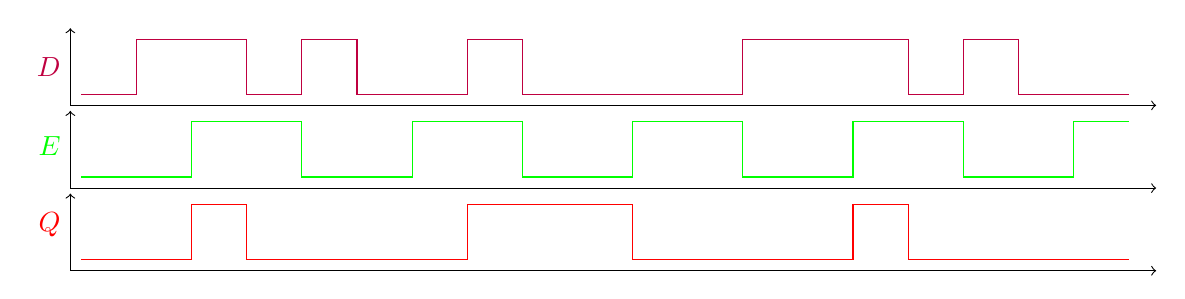
\begin{tikzpicture}[scale=0.7]
      \draw[<->] (-0.2, 1.2) -- (-0.2, -0.2) -- (19.5, -0.2); 
      \draw[<->, yshift=-1.5cm] (-0.2, 1.2) -- (-0.2, -0.2) -- (19.5, -0.2); 
      \draw[<->, yshift=-3cm] (-0.2, 1.2) -- (-0.2, -0.2) -- (19.5, -0.2); 
      \node[purple, left] at (-0.2, 0.5) {$D$}; 
      \node[green, left, yshift=-1cm] at (-0.2, 0.5) {$E$}; 
      \node[red, left, yshift=-2cm] at (-0.2, 0.5) {$Q$}; 

      \draw[purple] (0, 0) -- 
        (1, 0) -- (1, 1) -- (3, 1) -- (3, 0) -- 
        (4, 0) -- (4, 1) -- (5, 1) -- (5, 0) -- 
        (7, 0) -- (7, 1) -- (8, 1) -- (8, 0) -- 
        (12, 0) -- (12, 1) -- (15, 1) -- (15, 0) -- 
        (16, 0) -- (16, 1) -- (17, 1) -- (17, 0) -- 
        (19, 0);
      \draw[green, yshift=-1.5cm] (0, 0) -- 
        (2, 0) -- (2, 1) -- (4, 1) -- (4, 0) -- 
        (6, 0) -- (6, 1) -- (8, 1) -- (8, 0) -- 
        (10, 0) -- (10, 1) -- (12, 1) -- (12, 0) -- 
        (14, 0) -- (14, 1) -- (16, 1) -- (16, 0) -- 
        (18, 0) -- (18, 1) -- (19, 1);
      \draw[red, yshift=-3cm] (0, 0) -- 
        (2, 0) -- (2, 1) -- (3, 1) -- (3, 0) -- 
        (7, 0) -- (7, 1) -- (10, 1) -- (10, 0) -- 
        (14, 0) -- (14, 1) -- (15, 1) -- (15, 0) -- 
        (19, 0);
    \end{tikzpicture}
    \caption{$E$ is connected to a clock that ocsillates at regular intervals.}
  \end{figure}

  This is still not a perfect solution for synchronizing some components. Depending on the frequency of the clock, $E$ may be high for as long at 50 microseconds. That's a long time for the data latch to be open to changes in $D$. For some applications, particularly those where the outputs are fed back to the inputs, we can avoid disorder and noise from $D$ by drastically limiting the amount of time $E$ is open during each clock cycle. 
  
  But simply increasing the frequency of the clock isn't a practical solution, given that a computer contains a mixture of fast and slow components. A more clever solution is to only allow changes to the latch when the clock input $E$ is changing from low to high. Due to propagation delay, this is indeed a feasible solution since the waveforms are not truly square waves. 

  \begin{definition}[Rising, Falling Edge]
    The period when a signal 
    \begin{enumerate}
      \item changes from $0$ to $1$ is called the \textbf{rising edge}. 
      \item changes from $1$ to $0$ is called the \textbf{falling edge}. 
    \end{enumerate}
    This usually takes a few nanoseconds. 

    \begin{figure}[H]
      \centering 
      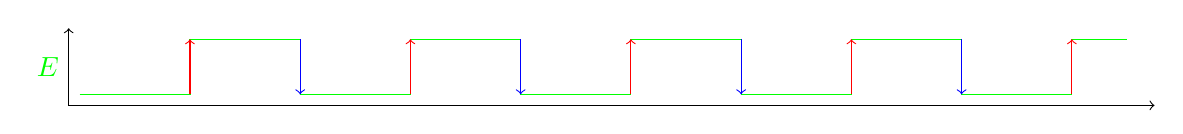
\begin{tikzpicture}[scale=0.7]
        \draw[<->] (-0.2, 1.2) -- (-0.2, -0.2) -- (19.5, -0.2); 
        \node[green, left] at (-0.2, 0.5) {$E$}; 

        \draw[green] (0, 0) -- 
          (2, 0) -- (2, 1) -- (4, 1) -- (4, 0) -- 
          (6, 0) -- (6, 1) -- (8, 1) -- (8, 0) -- 
          (10, 0) -- (10, 1) -- (12, 1) -- (12, 0) -- 
          (14, 0) -- (14, 1) -- (16, 1) -- (16, 0) -- 
          (18, 0) -- (18, 1) -- (19, 1);

        \draw[blue, <-] (4, 0) -- (4, 1); 
        \draw[blue, <-] (8, 0) -- (8, 1); 
        \draw[blue, <-] (12, 0) -- (12, 1); 
        \draw[blue, <-] (16, 0) -- (16, 1); 

        \draw[red, ->] (2, 0) -- (2, 1); 
        \draw[red, ->] (6, 0) -- (6, 1); 
        \draw[red, ->] (10, 0) -- (10, 1); 
        \draw[red, ->] (14, 0) -- (14, 1); 
        \draw[red, ->] (18, 0) -- (18, 1); 
      \end{tikzpicture}
      \caption{Rising edges are in red, falling edges in blue.}
    \end{figure}
  \end{definition}

  We want to build a D-latch that will respond to changes in $D$ \textit{at the rising edge}, with subsequent changes in $D$ being ignored until the next rising edge. 

  \begin{figure}[H]
    \centering
    \begin{subfigure}[b]{0.32\textwidth}
      \centering
      \begin{tikzpicture}[circuit logic US]
        \node[and gate, scale=1.5] (and) at (3, 0) {};
        \node[not gate] (not) at (1, -0.3) {};
        \draw[blue] (-1, 0.2) -- (0, 0.2) -- (0, -0.3) -- (not.input);
        \draw[red] (not.output) -- (and.input 2); 
        \draw[blue] (-1, 0.2) -- (and.input 1); 
        \draw[blue] (and.output) -- (4, 0);
        \fill[blue] (0, 0.2) circle (1.5pt);
      \end{tikzpicture}
      \caption{By default the input current is $0$, and so the top input of the AND gate is $0$ and the bottom is $1$. }
    \end{subfigure}
    \hfill 
    \begin{subfigure}[b]{0.32\textwidth}
      \centering
      \begin{tikzpicture}[circuit logic US]
        \node[and gate, scale=1.5] (and) at (3, 0) {};
        \node[not gate] (not) at (1, -0.3) {};
        \draw[red] (-1, 0.2) -- (0, 0.2) -- (0, -0.3) -- (not.input);
        \draw[red] (not.output) -- (and.input 2); 
        \draw[red] (-1, 0.2) -- (and.input 1); 
        \draw[red] (and.output) -- (4, 0);
        \fill[red] (0, 0.2) circle (1.5pt);
      \end{tikzpicture}
      \caption{If the electric current of $1$ travels through the input wire, the top AND input becomes $1$. There is a small delay where the current does not reach the output of the NOT gate, so the output is $1$. }
    \end{subfigure}
    \hfill 
    \begin{subfigure}[b]{0.32\textwidth}
      \centering
      \begin{tikzpicture}[circuit logic US]
        \node[and gate, scale=1.5] (and) at (3, 0) {};
        \node[not gate] (not) at (1, -0.3) {};
        \draw[red] (-1, 0.2) -- (0, 0.2) -- (0, -0.3) -- (not.input);
        \draw[blue] (not.output) -- (and.input 2); 
        \draw[red] (-1, 0.2) -- (and.input 1); 
        \draw[blue] (and.output) -- (4, 0);
        \fill[red] (0, 0.2) circle (1.5pt);
      \end{tikzpicture}
      \caption{The signal goes through the NOT gate, turning the AND output back to $0$.}
    \end{subfigure}
    \caption{An edge detection device. Note that if we want to delay the signal even further, we can put an arbitrary amount of NAND gates.}
  \end{figure}

  We take this idea to build an edge detection device. 

  \begin{definition}[Edge Detection Device]
    This is a rising edge detection device. Note that depending on many factors, like manufacturing, temperature, etc., there may not be a long enough delay to actually detect an edge, and in this case you can just add more (odd number of ) NOT gates 

    \begin{figure}[H]
      \centering
      \begin{subfigure}[b]{0.48\textwidth}
        \centering
        \begin{tikzpicture}[circuit logic US]
          \node[and gate, scale=1.5] (and) at (3, 0) {};
          \node[not gate] (not) at (1, -0.3) {};
          \draw (-1, 0.2) -- (0, 0.2) -- (0, -0.3) -- (not.input);
          \draw (not.output) -- (and.input 2); 
          \draw (-1, 0.2) -- (and.input 1); 
          \draw (and.output) -- (4, 0);
          \fill (0, 0.2) circle (1.5pt);
        \end{tikzpicture}
        \caption{Positive edge triggered detection device.}
      \end{subfigure}
      \hfill 
      \begin{subfigure}[b]{0.48\textwidth}
        \centering
        \begin{tikzpicture}[circuit logic US]
          \node[nor gate, scale=1.5] (and) at (3, 0) {};
          \node[not gate] (not) at (1, -0.3) {};
          \draw (-1, 0.2) -- (0, 0.2) -- (0, -0.3) -- (not.input);
          \draw (not.output) -- (and.input 2); 
          \draw (-1, 0.2) -- (and.input 1); 
          \draw (and.output) -- (4, 0);
          \fill (0, 0.2) circle (1.5pt);
        \end{tikzpicture}
        \caption{Negative edge triggered detection device.}
      \end{subfigure}
      \caption{}
    \end{figure}

    It has the following waveform. 

    \begin{figure}[H]
      \centering 
      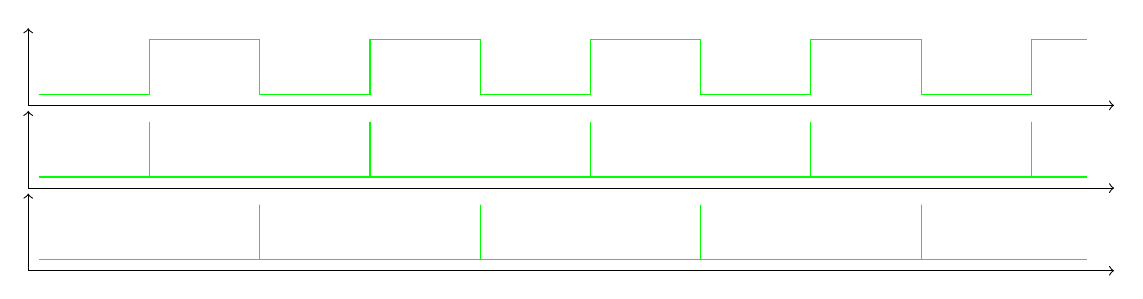
\begin{tikzpicture}[scale=0.7]
        \draw[<->] (-0.2, 1.2) -- (-0.2, -0.2) -- (19.5, -0.2); 
        \draw[<->, yshift=-1.5cm] (-0.2, 1.2) -- (-0.2, -0.2) -- (19.5, -0.2); 
        \draw[<->, yshift=-3cm] (-0.2, 1.2) -- (-0.2, -0.2) -- (19.5, -0.2); 

        \draw[green] (0, 0) -- 
          (2, 0) -- (2, 1) -- (4, 1) -- (4, 0) -- 
          (6, 0) -- (6, 1) -- (8, 1) -- (8, 0) -- 
          (10, 0) -- (10, 1) -- (12, 1) -- (12, 0) -- 
          (14, 0) -- (14, 1) -- (16, 1) -- (16, 0) -- 
          (18, 0) -- (18, 1) -- (19, 1);

        \draw[green, yshift=-1.5cm] (0, 0) -- 
          (2, 0) -- (2, 1) -- (2, 1) -- (2, 0) -- 
          (6, 0) -- (6, 1) -- (6, 1) -- (6, 0) -- 
          (10, 0) -- (10, 1) -- (10, 1) -- (10, 0) -- 
          (14, 0) -- (14, 1) -- (14, 1) -- (14, 0) -- 
          (18, 0) -- (18, 1) -- (18, 1) -- (18, 0) -- 
          (19, 0);

        \draw[green, yshift=-3cm] (0, 0) -- 
          (4, 0) -- (4, 1) -- (4, 0) -- 
          (8, 0) -- (8, 1) -- (8, 0) -- 
          (12, 0) -- (12, 1) -- (12, 0) -- 
          (16, 0) -- (16, 1) -- (16, 0) -- 
          (19, 0);
      \end{tikzpicture}
      \caption{The clock cycle (top). Positive edge detection device (middle). Negative edge detection device (bottom). }
    \end{figure}
  \end{definition}

  Now if we combine our D latch with the edge detection device, we change it from a level-triggered device to an edge-triggered device. Since we are using a clock as our trigger, we also call this a \textit{clocked D-latch}. 

  \begin{definition}[Clocked D Latch]
    A \textbf{clocked D latch}, also called an \textbf{edge-triggered D-latch},\footnote{Sometimes, this is referred to as a flip flop, but we will distinguish that a bit later.} is a D-latch that is enabled on the rising edge of a clock cycle. 

    \begin{figure}[H]
      \centering 
      \begin{tikzpicture}[circuit logic US]
        \node[flipflop D] (D1){};
      \end{tikzpicture}
      \caption{A pulse D latch. Note that the triangle is used to indicate that the clock is inputted. } 
    \end{figure}

    \begin{figure}[H]
      \centering 
      \begin{tikzpicture}[circuit logic US]
        \node[and gate] (and) at (-4, -1.2) {};
        \node[not gate, scale=0.7] (not) at (-5.3, -1.4) {};
        \draw (-6.2, -1.11) -- (and.input 1);
        \draw (-5.8, -1.11) -- (-5.8, -1.4) -- (not.input);
        \fill (-5.8, -1.11) circle (1.5pt); 
        \node[left] at (-6.2, -1.1) {CLK}; 
        \draw(and.output) -- (-3.2, -1.2);
        \draw(not.output) -- (and.input 2); 

        \node[nand gate] (nand1) at (-2, 1.1) {};
        \node[nand gate] (nand2) at (-2, -1.1) {};
        \node[nand gate] (nor1) at (0, 1) {}; 
        \node[nand gate] (nor2) at (0, -1) {}; 

        \draw (-3.5, 1.2) -- (nand1.input 1);
        \draw (-3.5, -1.2) -- (nand2.input 2);
        \node[left] at (-3.5,1.2) {$R$};
        \node[right] at (2, 1) {$Q$};
        \node[right] at (2, -1) {$\overline{Q}$};

        \draw (-3.5, -1.2) -- (-3.2, -1.2) -- (-3.2, 1) -- (nand1.input 2);
        \fill (-3.2, -1.2) circle (1.5pt);
        \draw (nand1.output) -- (-1.2, 1.1) -- (-1.2, 0.9) -- (-2.7, -0.9) -- (-2.7, -1) -- (nand2.input 1);

        \draw (nand1.output) -- (nor1.input 1);
        \draw (nand2.output) -- (nor2.input 2);
        \draw (nor1.output) -- (2, 1); 
        \draw (nor2.output) -- (2, -1); 

        \draw (nor1.output) -- (1.5, 1) -- (1.5, 0.8) -- (-1, -0.7) -- (-1, -0.9) -- (nor2.input 1);
        \draw (nor2.output) -- (1.5, -1) -- (1.5, -0.8) -- (-1, 0.7) -- (-1, 0.9) -- (nor1.input 2);
        \fill (1.5,1) circle (1.5pt);
        \fill (1.5,-1) circle (1.5pt);
      \end{tikzpicture} 
      \caption{} 
    \end{figure}
  \end{definition}

  \begin{example}[Clocked D Latch Waveforms]
    \begin{figure}[H]
      \centering 
      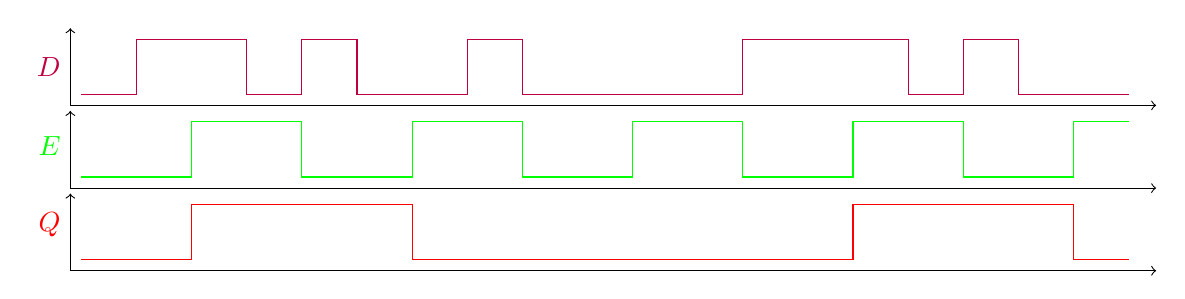
\begin{tikzpicture}[scale=0.7]
        \draw[<->] (-0.2, 1.2) -- (-0.2, -0.2) -- (19.5, -0.2); 
        \draw[<->, yshift=-1.5cm] (-0.2, 1.2) -- (-0.2, -0.2) -- (19.5, -0.2); 
        \draw[<->, yshift=-3cm] (-0.2, 1.2) -- (-0.2, -0.2) -- (19.5, -0.2); 
        \node[purple, left] at (-0.2, 0.5) {$D$}; 
        \node[green, left, yshift=-1cm] at (-0.2, 0.5) {$E$}; 
        \node[red, left, yshift=-2cm] at (-0.2, 0.5) {$Q$}; 

        \draw[purple] (0, 0) -- 
          (1, 0) -- (1, 1) -- (3, 1) -- (3, 0) -- 
          (4, 0) -- (4, 1) -- (5, 1) -- (5, 0) -- 
          (7, 0) -- (7, 1) -- (8, 1) -- (8, 0) -- 
          (12, 0) -- (12, 1) -- (15, 1) -- (15, 0) -- 
          (16, 0) -- (16, 1) -- (17, 1) -- (17, 0) -- 
          (19, 0);
        \draw[green, yshift=-1.5cm] (0, 0) -- 
          (2, 0) -- (2, 1) -- (4, 1) -- (4, 0) -- 
          (6, 0) -- (6, 1) -- (8, 1) -- (8, 0) -- 
          (10, 0) -- (10, 1) -- (12, 1) -- (12, 0) -- 
          (14, 0) -- (14, 1) -- (16, 1) -- (16, 0) -- 
          (18, 0) -- (18, 1) -- (19, 1);
        \draw[red, yshift=-3cm] (0, 0) -- 
          (2, 0) -- (2, 1) -- (6, 1) -- (6, 0) -- 
          (14, 0) -- (14, 1) -- (18, 1) -- (18, 0) --
          (19, 0);
      \end{tikzpicture}
      \caption{Again, we just let the result $Q$ follow the input $D$ whenever $E = 1$,and continue the rest for when $E = 0$.}
    \end{figure}
  \end{example}

  \begin{definition}[Pulse Latch]
    Another enhancement we can make is to have an option to manually set the latch to be either $Q = 1$ or $0$, independent of the clock. This gives us the \textbf{pulse D-latch}, which allows us to initialize it unconditionally. 

    \begin{figure}[H]
      \centering 
      \begin{tikzpicture}
        \node[latch, align=center, add async SR] (latch) at (0,0) {};
        \draw (latch.pin 1) -- ++(-0.5,0) node[left] {};
        \draw (latch.pin 3) -- ++(-0.5,0) node[left] {};
        \draw (latch.pin 6) -- ++(0.5,0) node[right] {};
        \draw (latch.pin 4) -- ++(0.5,0) node[right] {};
      \end{tikzpicture}
      \caption{D latch with asynchronous set/reset.} 
    \end{figure}

    The implementation is to simply add extra inputs after the NAND gates. 

    \begin{figure}[H]
      \centering 
      \begin{tikzpicture}[circuit logic US]
        \node[and gate] (and) at (-4, -1.2) {};
        \node[not gate, scale=0.7] (not) at (-5.3, -1.4) {};
        \draw (-6.2, -1.11) -- (and.input 1);
        \draw (-5.8, -1.11) -- (-5.8, -1.4) -- (not.input);
        \fill (-5.8, -1.11) circle (1.5pt); 
        \node[left] at (-6.2, -1.1) {CLK}; 
        \draw(and.output) -- (-3.2, -1.2);
        \draw(not.output) -- (and.input 2); 

        \node[nand gate] (nand1) at (-2, 1.1) {};
        \node[nand gate] (nand2) at (-2, -1.1) {};
        \node[nand gate, number inputs=3] (nor1) at (0, 1) {}; 
        \node[nand gate, number inputs=3] (nor2) at (0, -1) {}; 

        \draw (-3.5, 1.2) -- (nand1.input 1);
        \draw (-3.5, -1.2) -- (nand2.input 2);
        \node[left] at (-3.5,1.2) {$R$};
        \node[right] at (2, 1) {$Q$};
        \node[right] at (2, -1) {$\overline{Q}$};

        \draw (-3.5, -1.2) -- (-3.2, -1.2) -- (-3.2, 1) -- (nand1.input 2);
        \fill (-3.2, -1.2) circle (1.5pt);
        \draw (nand1.output) -- (-1.2, 1.1) -- (-1.2, 0.9) -- (-2.7, -0.9) -- (-2.7, -1) -- (nand2.input 1);

        \node[above] at (-1.2, 1.8) {SET};
        \node[below] at (-1.2, -1.8) {RESET};
        \draw (-1.2, 1.8) -- (-1.2, 1.2) -- ([yshift=0.1cm]nor1.input 1);
        \draw (-1.2, -1.8) -- (-1.2, -1.2) -- ([yshift=-0.1cm]nor2.input 2);
        \draw (nand1.output) -- (nor1.input 1);
        \draw (nand2.output) -- (nor2.input 2);
        \draw (nor1.output) -- (2, 1); 
        \draw (nor2.output) -- (2, -1); 

        \draw (nor1.output) -- (1.5, 1) -- (1.5, 0.8) -- (-1, -0.7) -- (-1, -0.9) -- (nor2.input 1);
        \draw (nor2.output) -- (1.5, -1) -- (1.5, -0.8) -- (-1, 0.7) -- (-1, 0.9) -- (nor1.input 2);
        \fill (1.5,1) circle (1.5pt);
        \fill (1.5,-1) circle (1.5pt);
      \end{tikzpicture} 
      \caption{} 
    \end{figure}
  \end{definition}

  This gives us a reliable device for storing 1 bit of memory. It is enabled and disabled by a clock signal, and used in registers, memory circuits, and counters as we will see later. 

\subsection{Flip Flops}

  So far, we have considered various mechanisms that allowed for greater control of a latch, along with robustness to noise. Now we revisit the final problem of attempting to \textit{coordinate} a group of latches. 

  \begin{figure}[H]
    \centering 
    \begin{tikzpicture}
      \node[draw, circle] (clock) at (-4, -1) {clock};
      \foreach \h in {0, 2, 4} {
        \node[flipflop D, scale=0.5] (D1) at (0.4, 0.6+\h){};
        \draw (D1.pin 3) -- ++(-0.85, 0) -- (-1, -1) -- (clock.east);
        \draw (D1.pin 1) -- ++ (-3, 0);
      }
    \end{tikzpicture}
    \caption{The ideal situation is that all the signals into $D$ will arrive, and then the next clock cycle begins, allowing each of the D-latches to update their states.} 
  \end{figure}

  There are new problems when considering a group of latches. First, there are many fast and slow moving parts of a computer. Therefore, we must wait for all wires to arrive---which may be a long time due to propagation delay---before we want to update the group of D-latches. Otherwise, the saved input would be garbage. To fix this, we could just decrease the frequency 

  \begin{definition}[Master-Slave D-Type Flip Flop]
    The \textbf{master-slave D-Type flip-flop}, we can precisely control the moment at which a group of them will change state. 

    \begin{figure}[H]
      \centering 
      \begin{tikzpicture}[circuit logic US]
        \begin{scope}[xshift=5cm]
          \node[nand gate] (nand13) at (-2, 1.1) {};
          \node[nand gate] (nand24) at (-2, -1.1) {};
          \node[nand gate] (nand14) at (0, 1) {}; 
          \node[nand gate] (nand23) at (0, -1) {}; 
          \draw (-3, 1.2) -- (nand13.input 1);
          \draw (-3, -1.2) -- (nand24.input 2);
          \draw (-8.2, -1.2) -- (-8.2, -1.7) -- (-3.3, -1.7) -- (-3.3, 0) -- (-2.7, 0) -- (-2.7,1) -- (nand13.input 2);
          \draw (-3, 0) -- (-2.7, 0) -- (-2.7,-1) -- (nand24.input 1);
          \node[right] at (2, 1) {$Q$};
          \node[right] at (2, -1) {$\overline{Q}$};
          \draw (nand13.output) -- (nand14.input 1);
          \draw (nand24.output) -- (nand23.input 2);
          \draw (nand14.output) -- (2, 1); 
          \draw (nand23.output) -- (2, -1); 
          \draw (nand14.output) -- (1.5, 1) -- (1.5, 0.8) -- (-1, -0.7) -- (-1, -0.9) -- (nand23.input 1);
          \draw (nand23.output) -- (1.5, -1) -- (1.5, -0.8) -- (-1, 0.7) -- (-1, 0.9) -- (nand14.input 2);
          \fill (1.5,1) circle (1.5pt);
          \fill (1.5,-1) circle (1.5pt);
          \fill (-2.7,0) circle (1.5pt);
        \end{scope}

        \node[nand gate] (nand1) at (-2, 1.1) {};
        \node[nand gate] (nand2) at (-2, -1.1) {};
        \node[nand gate] (nor1) at (0, 1) {}; 
        \node[nand gate] (nor2) at (0, -1) {}; 

        \draw (-3.5, 1.2) -- (nand1.input 1);
        \draw (-3.5, -1.2) -- (nand2.input 2);
        \node[left] at (-3.5,-1.2) {CLK};
        \node[left] at (-3.5,1.2) {$D$};

        \draw (-3.5, -1.2) -- (-3.2, -1.2) -- (-3.2, 1) -- (nand1.input 2);
        \fill (-3.2, -1.2) circle (1.5pt);
        \draw (nand1.output) -- (-1.2, 1.1) -- (-1.2, 0.9) -- (-2.7, -0.9) -- (-2.7, -1) -- (nand2.input 1);

        \draw (nand1.output) -- (nor1.input 1);
        \draw (nand2.output) -- (nor2.input 2);
        \draw (nor1.output) -- (2, 1) -- (2, 1.2); 
        \draw (nor2.output) -- (2, -1) -- (2, -1.2); 

        \draw (nor1.output) -- (1.5, 1) -- (1.5, 0.8) -- (-1, -0.7) -- (-1, -0.9) -- (nor2.input 1);
        \draw (nor2.output) -- (1.5, -1) -- (1.5, -0.8) -- (-1, 0.7) -- (-1, 0.9) -- (nor1.input 2);
        \fill (1.5,1) circle (1.5pt);
        \fill (1.5,-1) circle (1.5pt);
      \end{tikzpicture} 
      \caption{} 
    \end{figure}
  \end{definition}


  The most elementary chip is called a \textit{flip-flop}, of which there are many variants. In here, we will work with the data flip-flop. 

  \begin{definition}[Flip-Flop]
    A \textbf{data flip-flop (DFF)} is a device whose interface consists of a single-bit data input and single-bit data output. It also has a clock input that continuously changes accordingly to the master clock's signal. Taken together, the data and the clock inputs enable to the DFF to implement the time-based behavior 
    \begin{equation}
      \mathrm{out}(t) = \mathrm{in}(t - 1) 
    \end{equation}
    That is, the DFF outputs the input value from the previous time unit. 
  \end{definition}

\subsection{Registers}

  To understand anything that the CPU does, we must understand assembly language. In here, everything is done within registers, and we can see how the CPU fetches, decodes, and executes instructions. So what exactly are these registers? 

  \begin{definition}[Register]
    A register is a small, fast storage location within the CPU. It is used to store data that is being used immediately, and is the only place where the CPU can perform operations, which is why it must move data from memory to registers before it can perform operations on it. Everything in a register is in binary, at most 8 bytes, or 64 bits. 

    There are very specific types of registers that you should know. All of these registers are implemented for all assembly languages and are integral to the workflow of the CPU.  
    \begin{enumerate}
      \item \textbf{parameter registers} which store the parameters of a function.
      \item \textbf{Return registers} which store return values of functions. 
      \item \textbf{stack pointers} which point to the top of the stack (at the top of the current stack frame). 
      \item \textbf{frame pointers} which point to the base of the current stack frame.
      \item \textbf{instruction pointers} which point to the next instruction to be executed.
    \end{enumerate}
  \end{definition}

  \begin{definition}[32 and 64 Bit Machines]
    There are two types of machines that tend to format these boxes very differently: 32-bit and 64-bit machines. 
    \begin{enumerate}
      \item 32 bit machines store addresses in 32 bits, so they can have $2^{32}$ addresses, which is about 4 GB of memory. 
      \item 64 bit machines store addresses in 64 bits, so they can have $2^{64}$ addresses, which is about 16 EB of memory. This does not mean that the actual RAM is 16 EB, but it means that the machine can \textit{handle} that much memory. 
      \begin{lstlisting} 
        ...
        0x00007FFF7FBFF860 --> 0b000000000000000000000000011111111111
                               111101111111101111111111100001100000
        0x00007FFF7FBFF861 --> 0b000000000000000000000000011111111111
                               111101111111101111111111100001100001
        0x00007FFF7FBFF862 --> 0b000000000000000000000000011111111111
                               111101111111101111111111100001100010
        0x00007FFF7FBFF863 --> 0b000000000000000000000000011111111111
                               111101111111101111111111100001100011
        0x00007FFF7FBFF864 --> 0b000000000000000000000000011111111111
                               111101111111101111111111100001100100
        ...
      \end{lstlisting}
    \end{enumerate}
    The numbers typically mean the size of the type that the machine works best with, so all memory addresses will be 32 or 64 bits wide. Most machines are 64-bits, and so everything in this notes will assume that we are working with a 64 bit machine. As we will later see, this is why pointers are 8 bytes long, i.e. 64 bits. This is because the memory addresses are 64 bits long, though all of them are not used. 
  \end{definition}

\subsection{Memory Banks}

  \begin{definition}[Memory]
    The \textbf{memory} is where the computer stores data and instructions, which can be though of as a giant array of memory addresses, with each containing a byte. This data consists of graphical things or even instructions to manipulate other data. It can be visualized  as a long array of boxes that each have an \textbf{address} (where it is located) and \textbf{contents} (what is stored in it).

    Memory simply works as a bunch of bits in your computer with each bit having some memory address, which is also a bit. For example, the memory address \texttt{0b0010} (2) may have the bit value of \texttt{0b1} (1) stored in it. 

    \begin{figure}[H]
      \centering 
      \includegraphics[scale=0.4]{img/memory_visual_bit.png}
      \caption{Visualization of memory as a long array of boxes of bits. }
      \label{fig:memory_visual_bit}
    \end{figure}

    However, computers do not need this fine grained level of control on the memory, and they really work at the Byte level rather than the bit level. Therefore, we can visualize the memory as a long array of boxes indexed by \textit{Bytes}, with each value being a byte as well. In short, the memory is \textbf{byte-addressable}. In certain arthitectures, some systems are \textbf{word-addressable}, meaning that the memory is addressed by words, which are 4 bytes.\footnote{Note that in here the size of a word is 2 bytes rather than 4 as stated above. This is just how it is defined in some \texttt{x86} architectures.}

    \begin{figure}[H]
      \centering 
      \includegraphics[scale=0.4]{img/memory_visual_byte.png}
      \caption{Visualization of memory as a long array of boxes of bytes. Every address is a byte and its corresponding value at that address is also a byte, though we represent it as a 2-digit hex. } 
      \label{fig:memory_visual_byte}
    \end{figure}
  \end{definition}

  It is intuitive to think that given some multi-byte object like an \texttt{int} (4 bytes), the beginning of the int would be the lowest address and the end of the int would be the highest address, like how consecutive integers are stored in an array. However, this is not always the case (almost always not the case since most computers are little-endian).  

  \begin{definition}[Endian Architecture]
    Depending on the machine architecture, computers may store these types slightly differently in their \textit{byte} order. Say that we have an integer of value \texttt{0xA1B2C3D4} (4 bytes). Then, 
    \begin{enumerate} 
      \item A \textbf{big-endian architecture} (e.g. SPARC, z/Architecture) will store it so that the least significant byte has the highest address.
      \item A \textbf{little-endian architecture} (e.g. x86, x86-64, RISC-V) will store it so that the least significant byte has the lowest address. 
      \item A \textbf{bi-endian architecture} (e.g. ARM, PowerPC) can specify the endianness as big or little. 
    \end{enumerate}

    \begin{figure}[H]
      \centering 
      \includegraphics[scale=0.4]{img/endianness.png}
      \caption{The big vs little endian architectures. } 
      \label{fig:endianness}
    \end{figure}
  \end{definition}

  We can simply print out the hex values of primitive types to see how they are stored in memory, but it does not provide the level of details that we want on which bytes are stored where. At this point, we must use certain \textbf{debuggers} to directly look at the memory. For x86 architectures, we can use \texttt{gdb} and for ARM architectures, we can use \texttt{lldb}. At this point, we need to understand assembly to look through debuggers, so we will provide the example here. 

  \begin{example}[Endianness of C Int in x86-64]
    To do. 
  \end{example}

  \begin{example}[Endianness of C Int in ARM64]
    To do. 
  \end{example}

\subsection{Counter Chips}
